% Options for packages loaded elsewhere
\PassOptionsToPackage{unicode}{hyperref}
\PassOptionsToPackage{hyphens}{url}
%
\documentclass[
  ignorenonframetext,
]{beamer}
\usepackage{pgfpages}
\setbeamertemplate{caption}[numbered]
\setbeamertemplate{caption label separator}{: }
\setbeamercolor{caption name}{fg=normal text.fg}
\beamertemplatenavigationsymbolsempty
% Prevent slide breaks in the middle of a paragraph
\widowpenalties 1 10000
\raggedbottom
\setbeamertemplate{part page}{
  \centering
  \begin{beamercolorbox}[sep=16pt,center]{part title}
    \usebeamerfont{part title}\insertpart\par
  \end{beamercolorbox}
}
\setbeamertemplate{section page}{
  \centering
  \begin{beamercolorbox}[sep=12pt,center]{part title}
    \usebeamerfont{section title}\insertsection\par
  \end{beamercolorbox}
}
\setbeamertemplate{subsection page}{
  \centering
  \begin{beamercolorbox}[sep=8pt,center]{part title}
    \usebeamerfont{subsection title}\insertsubsection\par
  \end{beamercolorbox}
}
\AtBeginPart{
  \frame{\partpage}
}
\AtBeginSection{
  \ifbibliography
  \else
    \frame{\sectionpage}
  \fi
}
\AtBeginSubsection{
  \frame{\subsectionpage}
}
\usepackage{lmodern}
\usepackage{amssymb,amsmath}
\usepackage{ifxetex,ifluatex}
\ifnum 0\ifxetex 1\fi\ifluatex 1\fi=0 % if pdftex
  \usepackage[T1]{fontenc}
  \usepackage[utf8]{inputenc}
  \usepackage{textcomp} % provide euro and other symbols
\else % if luatex or xetex
  \usepackage{unicode-math}
  \defaultfontfeatures{Scale=MatchLowercase}
  \defaultfontfeatures[\rmfamily]{Ligatures=TeX,Scale=1}
\fi
\usetheme[]{Hannover}
\usecolortheme{dove}
\usefonttheme{structurebold}
% Use upquote if available, for straight quotes in verbatim environments
\IfFileExists{upquote.sty}{\usepackage{upquote}}{}
\IfFileExists{microtype.sty}{% use microtype if available
  \usepackage[]{microtype}
  \UseMicrotypeSet[protrusion]{basicmath} % disable protrusion for tt fonts
}{}
\makeatletter
\@ifundefined{KOMAClassName}{% if non-KOMA class
  \IfFileExists{parskip.sty}{%
    \usepackage{parskip}
  }{% else
    \setlength{\parindent}{0pt}
    \setlength{\parskip}{6pt plus 2pt minus 1pt}}
}{% if KOMA class
  \KOMAoptions{parskip=half}}
\makeatother
\usepackage{xcolor}
\IfFileExists{xurl.sty}{\usepackage{xurl}}{} % add URL line breaks if available
\IfFileExists{bookmark.sty}{\usepackage{bookmark}}{\usepackage{hyperref}}
\hypersetup{
  pdftitle={Session 8: Survival analysis part 3},
  pdfauthor={Levi Waldron},
  hidelinks,
  pdfcreator={LaTeX via pandoc}}
\urlstyle{same} % disable monospaced font for URLs
\newif\ifbibliography
\usepackage{color}
\usepackage{fancyvrb}
\newcommand{\VerbBar}{|}
\newcommand{\VERB}{\Verb[commandchars=\\\{\}]}
\DefineVerbatimEnvironment{Highlighting}{Verbatim}{commandchars=\\\{\}}
% Add ',fontsize=\small' for more characters per line
\usepackage{framed}
\definecolor{shadecolor}{RGB}{248,248,248}
\newenvironment{Shaded}{\begin{snugshade}}{\end{snugshade}}
\newcommand{\AlertTok}[1]{\textcolor[rgb]{0.94,0.16,0.16}{#1}}
\newcommand{\AnnotationTok}[1]{\textcolor[rgb]{0.56,0.35,0.01}{\textbf{\textit{#1}}}}
\newcommand{\AttributeTok}[1]{\textcolor[rgb]{0.77,0.63,0.00}{#1}}
\newcommand{\BaseNTok}[1]{\textcolor[rgb]{0.00,0.00,0.81}{#1}}
\newcommand{\BuiltInTok}[1]{#1}
\newcommand{\CharTok}[1]{\textcolor[rgb]{0.31,0.60,0.02}{#1}}
\newcommand{\CommentTok}[1]{\textcolor[rgb]{0.56,0.35,0.01}{\textit{#1}}}
\newcommand{\CommentVarTok}[1]{\textcolor[rgb]{0.56,0.35,0.01}{\textbf{\textit{#1}}}}
\newcommand{\ConstantTok}[1]{\textcolor[rgb]{0.00,0.00,0.00}{#1}}
\newcommand{\ControlFlowTok}[1]{\textcolor[rgb]{0.13,0.29,0.53}{\textbf{#1}}}
\newcommand{\DataTypeTok}[1]{\textcolor[rgb]{0.13,0.29,0.53}{#1}}
\newcommand{\DecValTok}[1]{\textcolor[rgb]{0.00,0.00,0.81}{#1}}
\newcommand{\DocumentationTok}[1]{\textcolor[rgb]{0.56,0.35,0.01}{\textbf{\textit{#1}}}}
\newcommand{\ErrorTok}[1]{\textcolor[rgb]{0.64,0.00,0.00}{\textbf{#1}}}
\newcommand{\ExtensionTok}[1]{#1}
\newcommand{\FloatTok}[1]{\textcolor[rgb]{0.00,0.00,0.81}{#1}}
\newcommand{\FunctionTok}[1]{\textcolor[rgb]{0.00,0.00,0.00}{#1}}
\newcommand{\ImportTok}[1]{#1}
\newcommand{\InformationTok}[1]{\textcolor[rgb]{0.56,0.35,0.01}{\textbf{\textit{#1}}}}
\newcommand{\KeywordTok}[1]{\textcolor[rgb]{0.13,0.29,0.53}{\textbf{#1}}}
\newcommand{\NormalTok}[1]{#1}
\newcommand{\OperatorTok}[1]{\textcolor[rgb]{0.81,0.36,0.00}{\textbf{#1}}}
\newcommand{\OtherTok}[1]{\textcolor[rgb]{0.56,0.35,0.01}{#1}}
\newcommand{\PreprocessorTok}[1]{\textcolor[rgb]{0.56,0.35,0.01}{\textit{#1}}}
\newcommand{\RegionMarkerTok}[1]{#1}
\newcommand{\SpecialCharTok}[1]{\textcolor[rgb]{0.00,0.00,0.00}{#1}}
\newcommand{\SpecialStringTok}[1]{\textcolor[rgb]{0.31,0.60,0.02}{#1}}
\newcommand{\StringTok}[1]{\textcolor[rgb]{0.31,0.60,0.02}{#1}}
\newcommand{\VariableTok}[1]{\textcolor[rgb]{0.00,0.00,0.00}{#1}}
\newcommand{\VerbatimStringTok}[1]{\textcolor[rgb]{0.31,0.60,0.02}{#1}}
\newcommand{\WarningTok}[1]{\textcolor[rgb]{0.56,0.35,0.01}{\textbf{\textit{#1}}}}
\usepackage{graphicx,grffile}
\makeatletter
\def\maxwidth{\ifdim\Gin@nat@width>\linewidth\linewidth\else\Gin@nat@width\fi}
\def\maxheight{\ifdim\Gin@nat@height>\textheight\textheight\else\Gin@nat@height\fi}
\makeatother
% Scale images if necessary, so that they will not overflow the page
% margins by default, and it is still possible to overwrite the defaults
% using explicit options in \includegraphics[width, height, ...]{}
\setkeys{Gin}{width=\maxwidth,height=\maxheight,keepaspectratio}
% Set default figure placement to htbp
\makeatletter
\def\fps@figure{htbp}
\makeatother
\setlength{\emergencystretch}{3em} % prevent overfull lines
\providecommand{\tightlist}{%
  \setlength{\itemsep}{0pt}\setlength{\parskip}{0pt}}
\setcounter{secnumdepth}{-\maxdimen} % remove section numbering

\title{Session 8: Survival analysis part 3}
\author{Levi Waldron}
\date{}
\institute{CUNY SPH Biostatistics 2}

\begin{document}
\frame{\titlepage}

\hypertarget{learning-objectives-and-outline}{%
\section{Learning objectives and
outline}\label{learning-objectives-and-outline}}

\begin{frame}{Learning objectives}
\protect\hypertarget{learning-objectives}{}

\begin{enumerate}
\tightlist
\item
  Check model assumptions and fit of the Cox model

  \begin{itemize}
  \tightlist
  \item
    residuals analysis
  \item
    log-minus-log plot
  \end{itemize}
\item
  Fit and interpret multivariate Cox models

  \begin{itemize}
  \tightlist
  \item
    perform tests for trend
  \item
    predict survival for specific covariate patterns
  \item
    predict survival for adjusted coefficients
  \end{itemize}
\item
  Explain stratified analysis
\item
  Identify situations of competing risks
\item
  Describe the application of Propensity Score analysis
\end{enumerate}

\begin{itemize}
\tightlist
\item
  Vittinghoff sections 6.2-6.4
\end{itemize}

\end{frame}

\begin{frame}{Outline}
\protect\hypertarget{outline}{}

\begin{enumerate}
\tightlist
\item
  Review
\item
  Assumptions of Cox PH model
\item
  Tests for trend
\item
  Predictions for specific covariate patterns
\item
  Stratification
\item
  Competing risks
\item
  Propensity Score analysis to control for confounding
\end{enumerate}

\end{frame}

\hypertarget{review}{%
\section{Review}\label{review}}

\begin{frame}{Cox proportional hazards model}
\protect\hypertarget{cox-proportional-hazards-model}{}

\begin{itemize}
\tightlist
\item
  Cox proportional hazard regression assesses the relationship between a
  right-censored, time-to-event outcome and multiple predictors:

  \begin{itemize}
  \tightlist
  \item
    categorical variables (e.g., treatment groups)
  \item
    continuous variables
  \end{itemize}
\end{itemize}

\[
log(HR(x_i)) = log \frac{h(t|x_i)}{h_0(t)} = \beta_0 + \beta_1 x_{1i} + \beta_2 x_{2i} + ... + \beta_p x_{pi}
\]

\begin{itemize}
\item
  \(HR(x_i)\) is the hazard of patient \(i\) relative to baseline
\item
  \(h(t|x_i)\) is the time-dependent hazard function \(h(t)\) for
  patient \(i\)
\item
  \(h_0(t)\) is the \emph{baseline hazard function}, and is the negative
  of the slope of the \(S_0(t)\), the baseline \emph{survival} function.
\item
  Multiplicative model
\end{itemize}

\end{frame}

\begin{frame}{Caveats and Assumptions}
\protect\hypertarget{caveats-and-assumptions}{}

\begin{itemize}
\tightlist
\item
  Categories with no events

  \begin{itemize}
  \tightlist
  \item
    can occur when the group is small or its risk is low
  \item
    HRs with respect to such a reference group are infinite
  \item
    hypothesis tests and CIs are difficult / impossible to interpret
  \end{itemize}
\item
  Assumptions of Cox PH model

  \begin{itemize}
  \tightlist
  \item
    Constant hazard ratio over time (proportional hazards)
  \item
    Linear association between log(HR) and predictors (log-linearity) /
    multiplicative relationship between hazard and predictors
  \item
    Independence of survival times between individuals in the sample
  \end{itemize}
\end{itemize}

\end{frame}

\hypertarget{checking-assumptions-of-cox-model}{%
\section{Checking assumptions of Cox
model}\label{checking-assumptions-of-cox-model}}

\begin{frame}[fragile]{Residuals analysis}
\protect\hypertarget{residuals-analysis}{}

\begin{itemize}
\tightlist
\item
  Residuals are used to investigate the lack of fit of a model to a
  given subject.
\item
  For Cox regression, there's no easy analog to the usual ``observed
  minus predicted'' residual
\end{itemize}

\footnotesize

\begin{Shaded}
\begin{Highlighting}[]
\KeywordTok{library}\NormalTok{(pensim)}
\KeywordTok{set.seed}\NormalTok{(}\DecValTok{1}\NormalTok{)}
\NormalTok{mydat <-}\StringTok{ }\KeywordTok{create.data}\NormalTok{(}
  \DataTypeTok{nvars =} \KeywordTok{c}\NormalTok{(}\DecValTok{1}\NormalTok{, }\DecValTok{1}\NormalTok{),}
  \DataTypeTok{nsamples =} \DecValTok{500}\NormalTok{,}
  \DataTypeTok{cors =} \KeywordTok{c}\NormalTok{(}\DecValTok{0}\NormalTok{, }\DecValTok{0}\NormalTok{),}
  \DataTypeTok{associations =} \KeywordTok{c}\NormalTok{(}\FloatTok{0.5}\NormalTok{, }\FloatTok{0.5}\NormalTok{),}
  \DataTypeTok{firstonly =} \KeywordTok{c}\NormalTok{(}\OtherTok{TRUE}\NormalTok{, }\OtherTok{TRUE}\NormalTok{),}
  \DataTypeTok{censoring =} \KeywordTok{c}\NormalTok{(}\DecValTok{0}\NormalTok{, }\FloatTok{8.5}\NormalTok{)}
\NormalTok{)}\OperatorTok{$}\NormalTok{data}
\end{Highlighting}
\end{Shaded}

\begin{Shaded}
\begin{Highlighting}[]
\CommentTok{## Rename variables of simulated data, and make one variable categorical.}
\KeywordTok{library}\NormalTok{(dplyr)}
\end{Highlighting}
\end{Shaded}

\begin{verbatim}
## 
## Attaching package: 'dplyr'
\end{verbatim}

\begin{verbatim}
## The following objects are masked from 'package:stats':
## 
##     filter, lag
\end{verbatim}

\begin{verbatim}
## The following objects are masked from 'package:base':
## 
##     intersect, setdiff, setequal, union
\end{verbatim}

\begin{Shaded}
\begin{Highlighting}[]
\NormalTok{mydat <-}\StringTok{ }\NormalTok{mydat }\OperatorTok\StringTok{ }\KeywordTok{rename}\NormalTok{(}\DataTypeTok{Var1 =}\NormalTok{ a}\FloatTok{.1}\NormalTok{, }\DataTypeTok{Var2 =}\NormalTok{ b}\FloatTok{.1}\NormalTok{) }\OperatorTok
\StringTok{  }\KeywordTok{mutate}\NormalTok{(}\DataTypeTok{Var1 =} \KeywordTok{cut}\NormalTok{(Var1,}
                    \DataTypeTok{breaks =} \DecValTok{2}\NormalTok{,}
                    \DataTypeTok{labels =} \KeywordTok{c}\NormalTok{(}\StringTok{"low"}\NormalTok{, }\StringTok{"high"}\NormalTok{)),}
         \DataTypeTok{time =} \KeywordTok{ceiling}\NormalTok{(time }\OperatorTok{*}\StringTok{ }\DecValTok{1000}\NormalTok{))}
\end{Highlighting}
\end{Shaded}

\end{frame}

\begin{frame}[fragile]{Simulated data to test residuals methods}
\protect\hypertarget{simulated-data-to-test-residuals-methods}{}

\footnotesize

\begin{Shaded}
\begin{Highlighting}[]
\KeywordTok{summary}\NormalTok{(mydat)}
\end{Highlighting}
\end{Shaded}

\begin{verbatim}
##    Var1          Var2               time           cens      
##  low :323   Min.   :-2.99695   Min.   :   5   Min.   :0.000  
##  high:177   1st Qu.:-0.79008   1st Qu.: 691   1st Qu.:0.000  
##             Median :-0.02126   Median :1970   Median :1.000  
##             Mean   :-0.04594   Mean   :2529   Mean   :0.526  
##             3rd Qu.: 0.68933   3rd Qu.:3874   3rd Qu.:1.000  
##             Max.   : 3.05574   Max.   :8481   Max.   :1.000
\end{verbatim}

\end{frame}

\begin{frame}[fragile]{Kaplan-Meier plot of simulated data, stratified
by Var1}
\protect\hypertarget{kaplan-meier-plot-of-simulated-data-stratified-by-var1}{}

\begin{verbatim}
## Loading required package: ggplot2
\end{verbatim}

\begin{verbatim}
## Loading required package: ggpubr
\end{verbatim}

\begin{verbatim}
## Warning: Vectorized input to `element_text()` is not officially supported.
## Results may be unexpected or may change in future versions of ggplot2.
\end{verbatim}

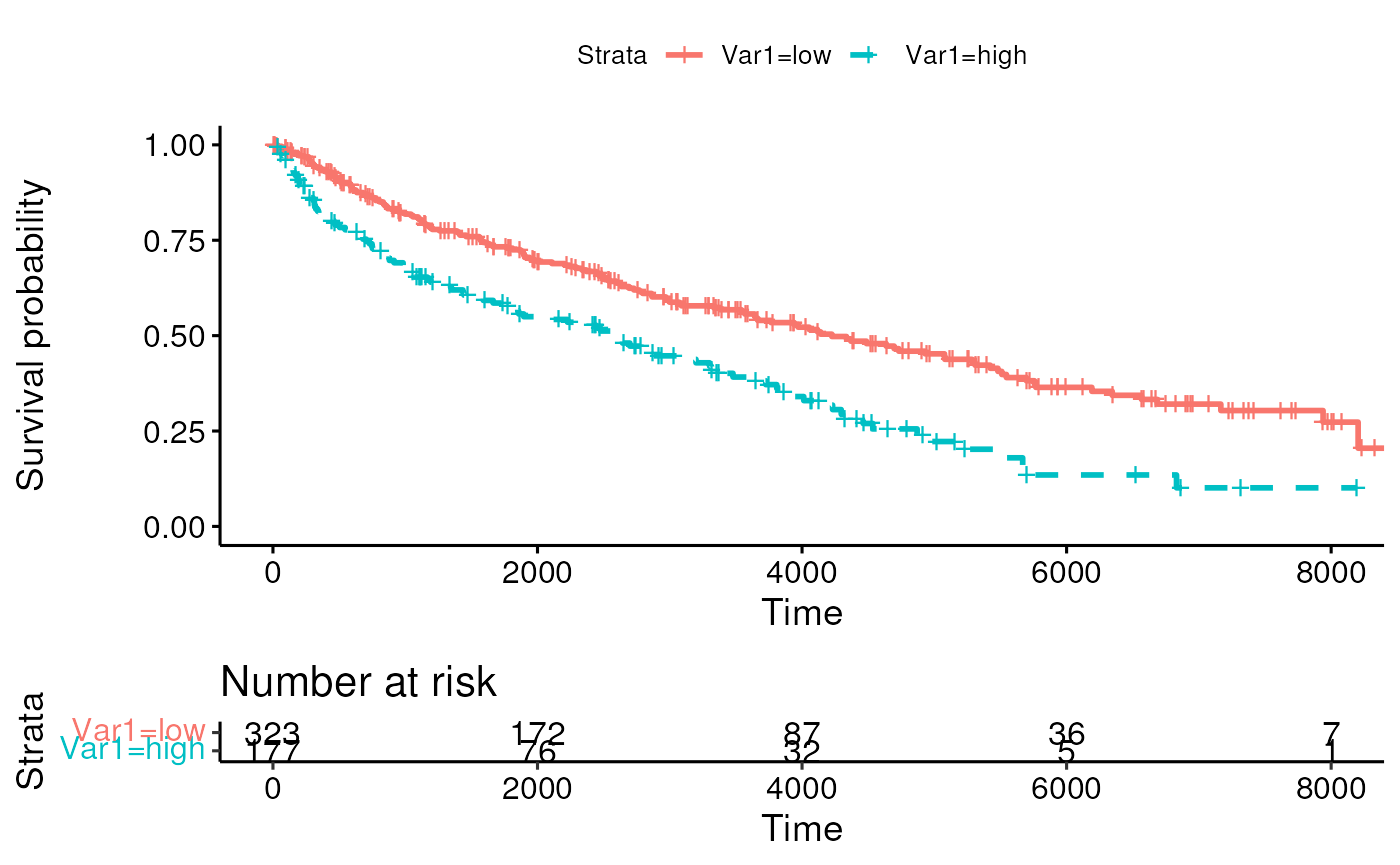
\includegraphics{../docs/articles/session_lecture_files/figure-beamer/unnamed-chunk-4-1.pdf}

\end{frame}

\begin{frame}{Martingale residuals}
\protect\hypertarget{martingale-residuals}{}

\begin{itemize}
\tightlist
\item
  censoring variable \(c_i\) (1 if event, 0 if censored) minus the
  estimated cumulative hazard function \(H(t_i, X_i, \beta_i)\) (1 -
  survival function)

  \begin{itemize}
  \tightlist
  \item
    E.g., for a subject censored at 1 year (\(c_i=0\)), whose predicted
    cumulative hazard at 1 year was 30\%, Martingale =
    \(0 - 0.30 = -0.30\).
  \item
    E.g. for a subject who had an event at 6 months, and whose predicted
    cumulative hazard at 6 months was 80\%, Margingale =
    \(1 - 0.8 = 0.2\).
  \end{itemize}
\item
  Problem: not symmetrically distributed, even when model fits the data
  well
\end{itemize}

\end{frame}

\begin{frame}{Martingale residuals in simulated data}
\protect\hypertarget{martingale-residuals-in-simulated-data}{}

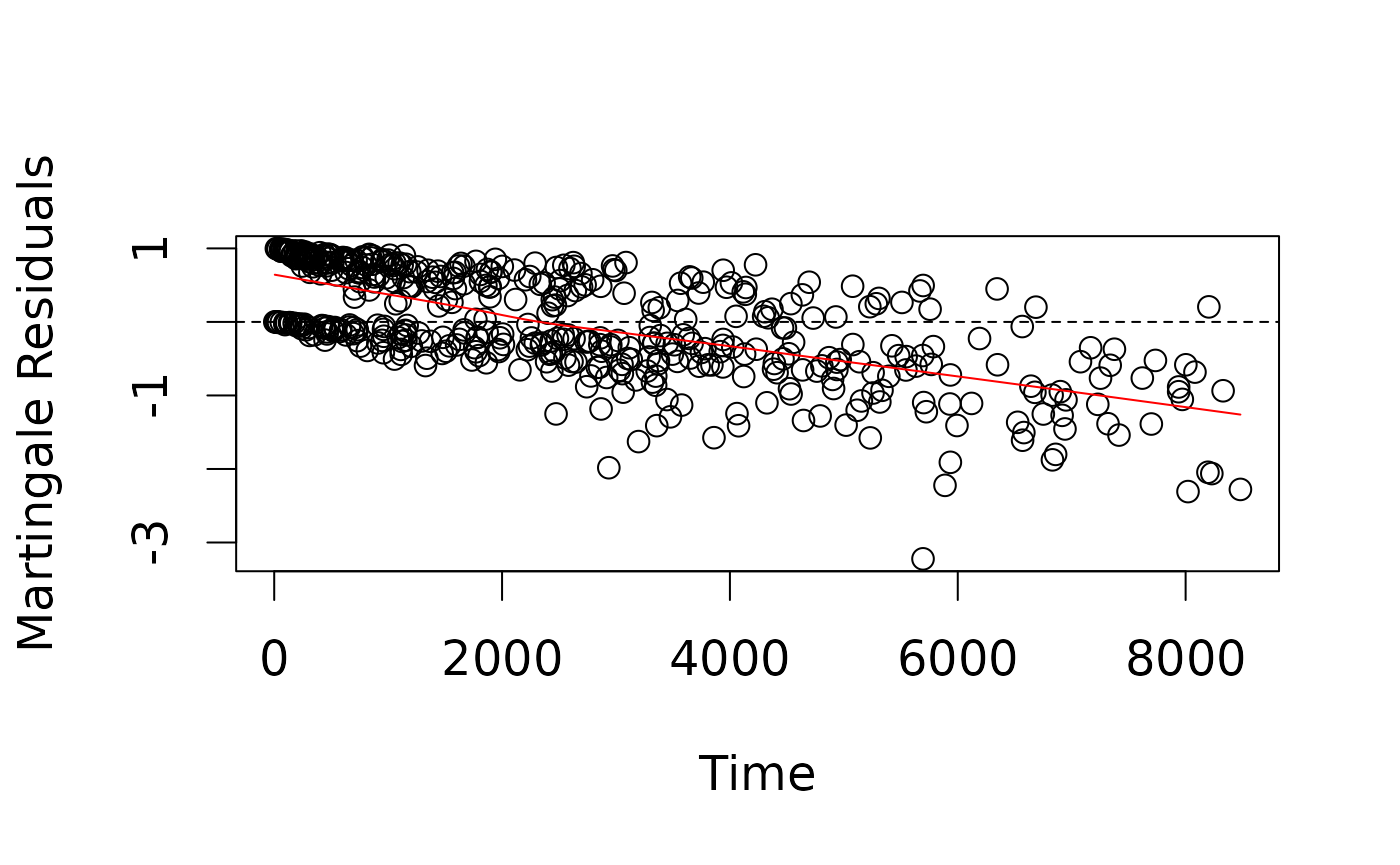
\includegraphics{../docs/articles/session_lecture_files/figure-beamer/unnamed-chunk-5-1.pdf}

\end{frame}

\begin{frame}{Deviance residuals in simulated data}
\protect\hypertarget{deviance-residuals-in-simulated-data}{}

\begin{itemize}
\tightlist
\item
  Deviance residuals are scaled Martingale residuals
\item
  Should be more symmetrically distributed about zero?
\item
  Observations with large deviance residuals are poorly predicted by the
  model
  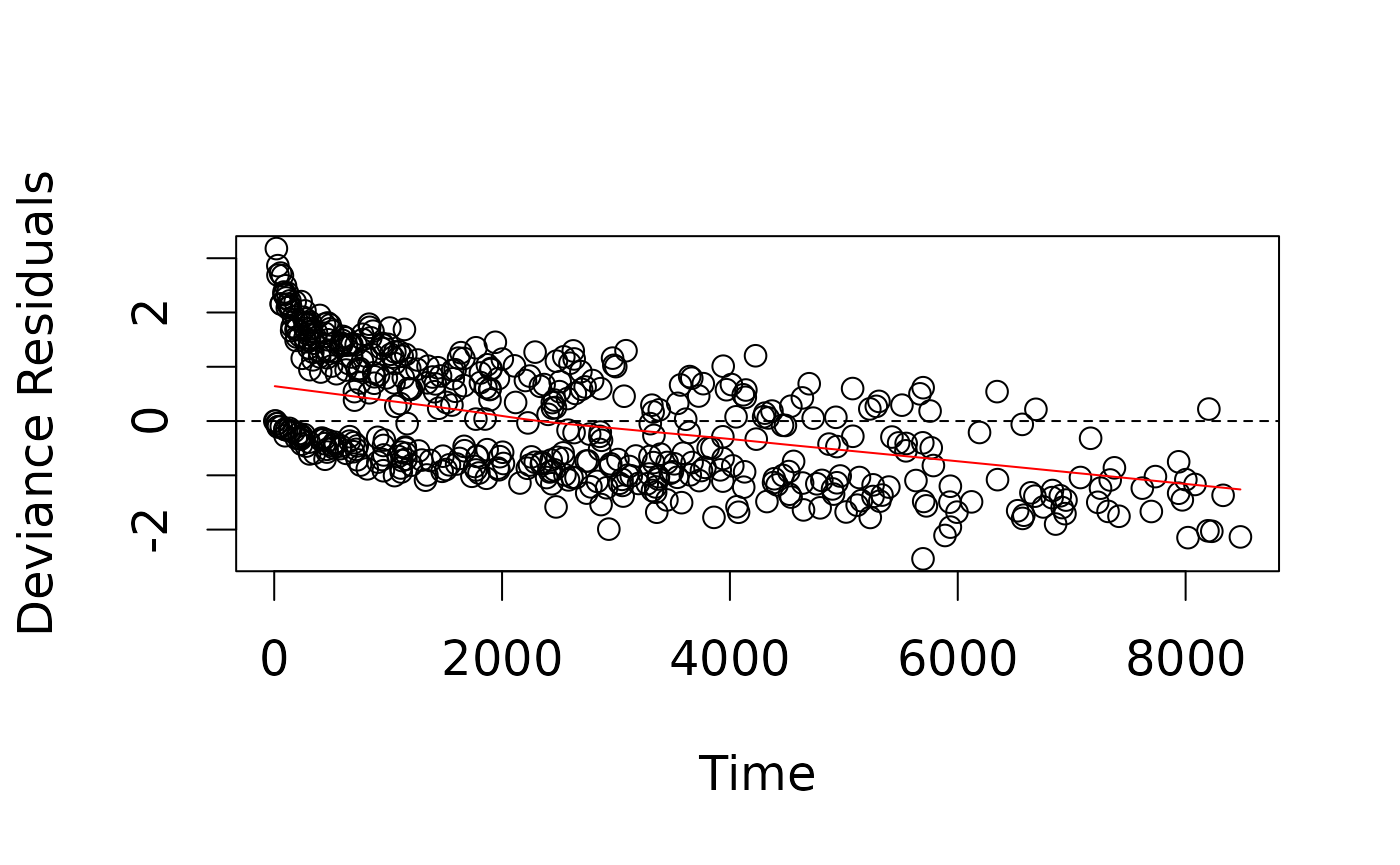
\includegraphics{../docs/articles/session_lecture_files/figure-beamer/unnamed-chunk-6-1.pdf}
\end{itemize}

\end{frame}

\begin{frame}{Schoenfeld residuals}
\protect\hypertarget{schoenfeld-residuals}{}

\begin{itemize}
\tightlist
\item
  technical definition: contribution of a covariate at each event time
  to the partial derivative of the log-likelihood
\item
  intuitive interpretation: the observed minus the expected values of
  the covariates at each event time.
\item
  a random (unsystematic) pattern across event times gives evidence the
  covariate effect is not changing with respect to time
\item
  If it is systematic, it suggests that as time passes, the covariate
  effect is changing.
\end{itemize}

\end{frame}

\begin{frame}{Schoenfeld residuals for simulated data}
\protect\hypertarget{schoenfeld-residuals-for-simulated-data}{}

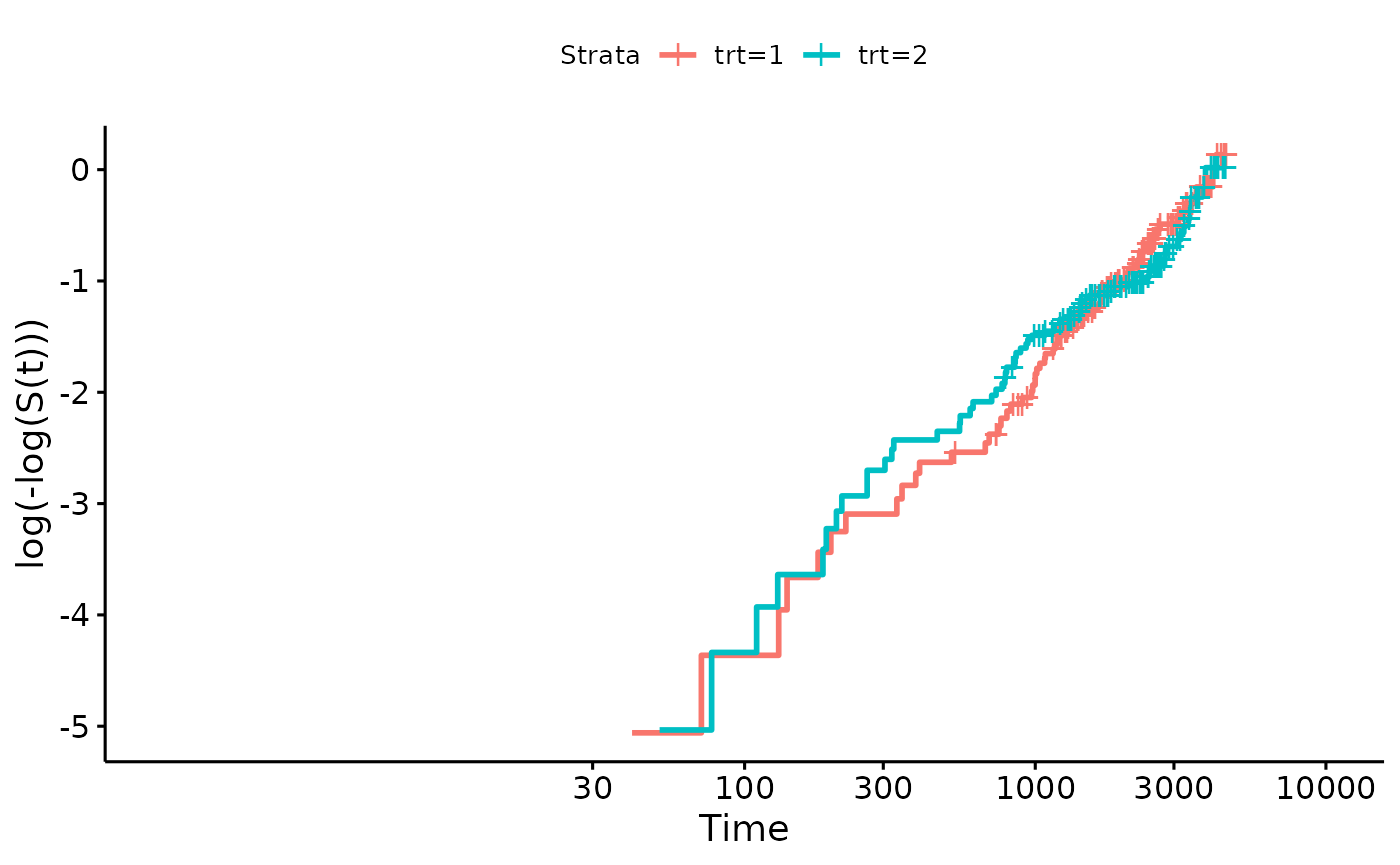
\includegraphics{../docs/articles/session_lecture_files/figure-beamer/unnamed-chunk-7-1.pdf}

\end{frame}

\begin{frame}[fragile]{Schoenfeld test for proportional hazards}
\protect\hypertarget{schoenfeld-test-for-proportional-hazards}{}

\begin{itemize}
\tightlist
\item
  Tests correlation between scaled Schoenfeld residuals and time
\item
  Equivalent to fitting a simple linear regression model with time as
  the predictor and residuals as the outcome
\item
  Parametric analog of smoothing the residuals against time using LOWESS
\item
  If the hazard ratio is constant, correlation should be zero.

  \begin{itemize}
  \tightlist
  \item
    Positive values of the correlation suggest that the log-hazard ratio
    increases with time.
  \end{itemize}
\end{itemize}

\begin{verbatim}
##          chisq df     p
## Var1   0.00887  1 0.925
## Var2   4.92734  1 0.026
## GLOBAL 5.07415  2 0.079
\end{verbatim}

\end{frame}

\begin{frame}{The hazard function h(t), stratified by Var1}
\protect\hypertarget{the-hazard-function-ht-stratified-by-var1}{}

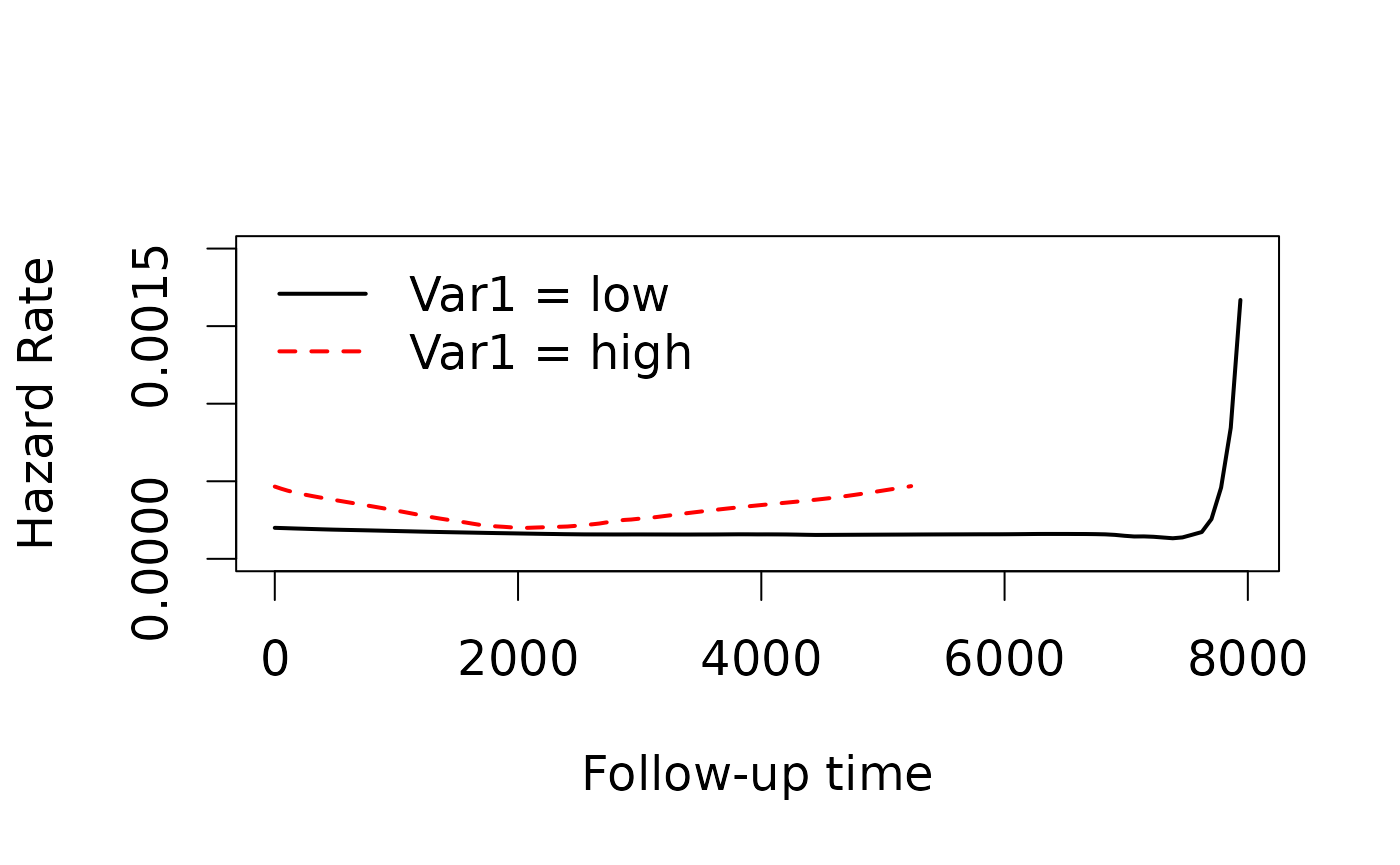
\includegraphics{../docs/articles/session_lecture_files/figure-beamer/unnamed-chunk-9-1.pdf}

\end{frame}

\begin{frame}{Log-minus-log plot}
\protect\hypertarget{log-minus-log-plot}{}

\begin{itemize}
\tightlist
\item
  Used to check proportional hazards assumption
\end{itemize}

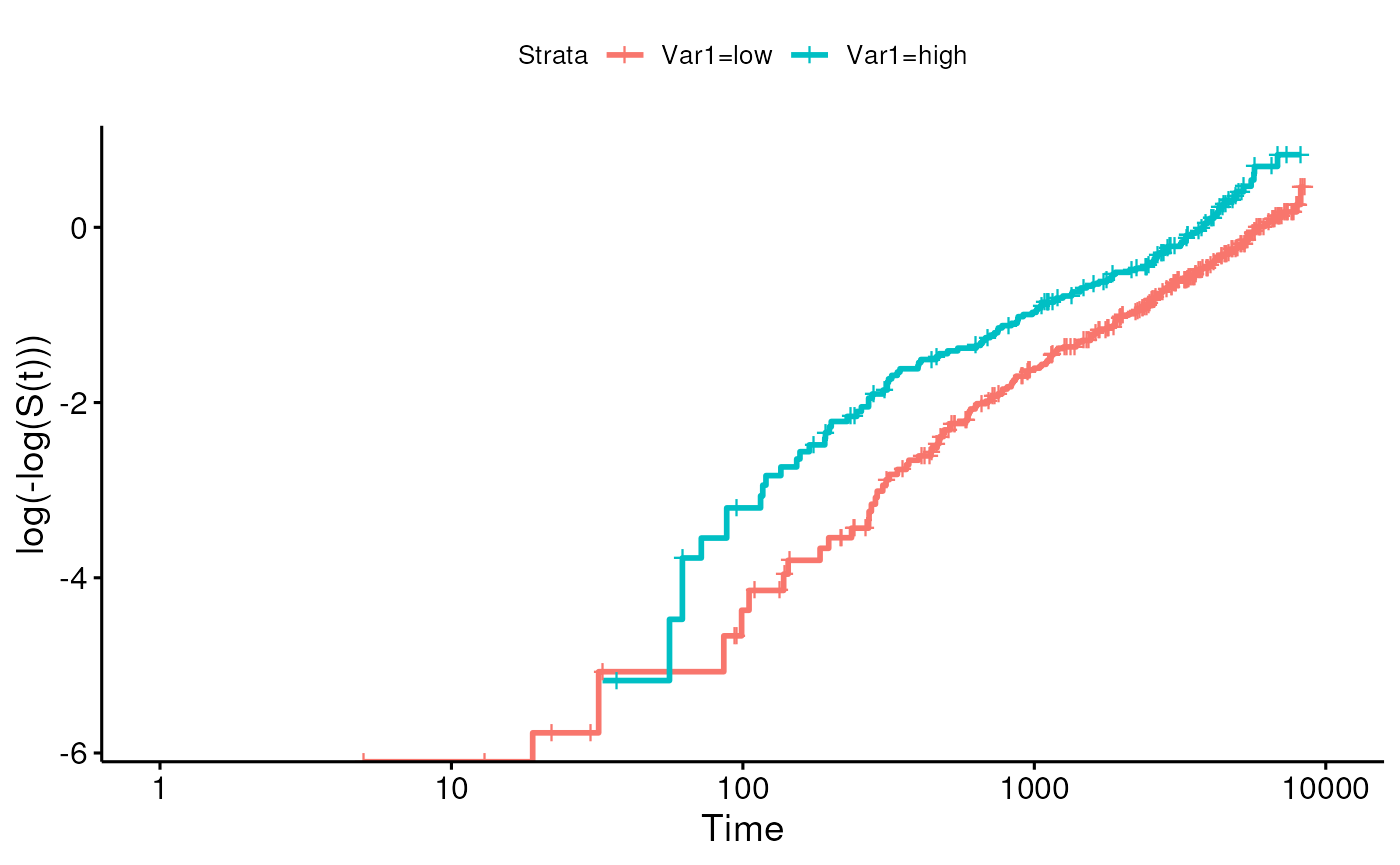
\includegraphics{../docs/articles/session_lecture_files/figure-beamer/unnamed-chunk-10-1.pdf}

\end{frame}

\begin{frame}{Example: Primary Biliary Cirrhosis (PBC)}
\protect\hypertarget{example-primary-biliary-cirrhosis-pbc}{}

\begin{itemize}
\tightlist
\item
  Mayo Clinic trial in primary biliary cirrhosis (PBC) of the liver
  conducted between 1974 and 1984, n=424 patients.
\item
  randomized placebo controlled trial of the drug D-penicillamine.

  \begin{itemize}
  \tightlist
  \item
    312 cases from RCT, plus additional 112 not from RCT.
  \end{itemize}
\item
  Primary outcome is (censored) time to death
\end{itemize}

\end{frame}

\begin{frame}[fragile]{Kaplan-Meier plot of treatment and placebo arms}
\protect\hypertarget{kaplan-meier-plot-of-treatment-and-placebo-arms}{}

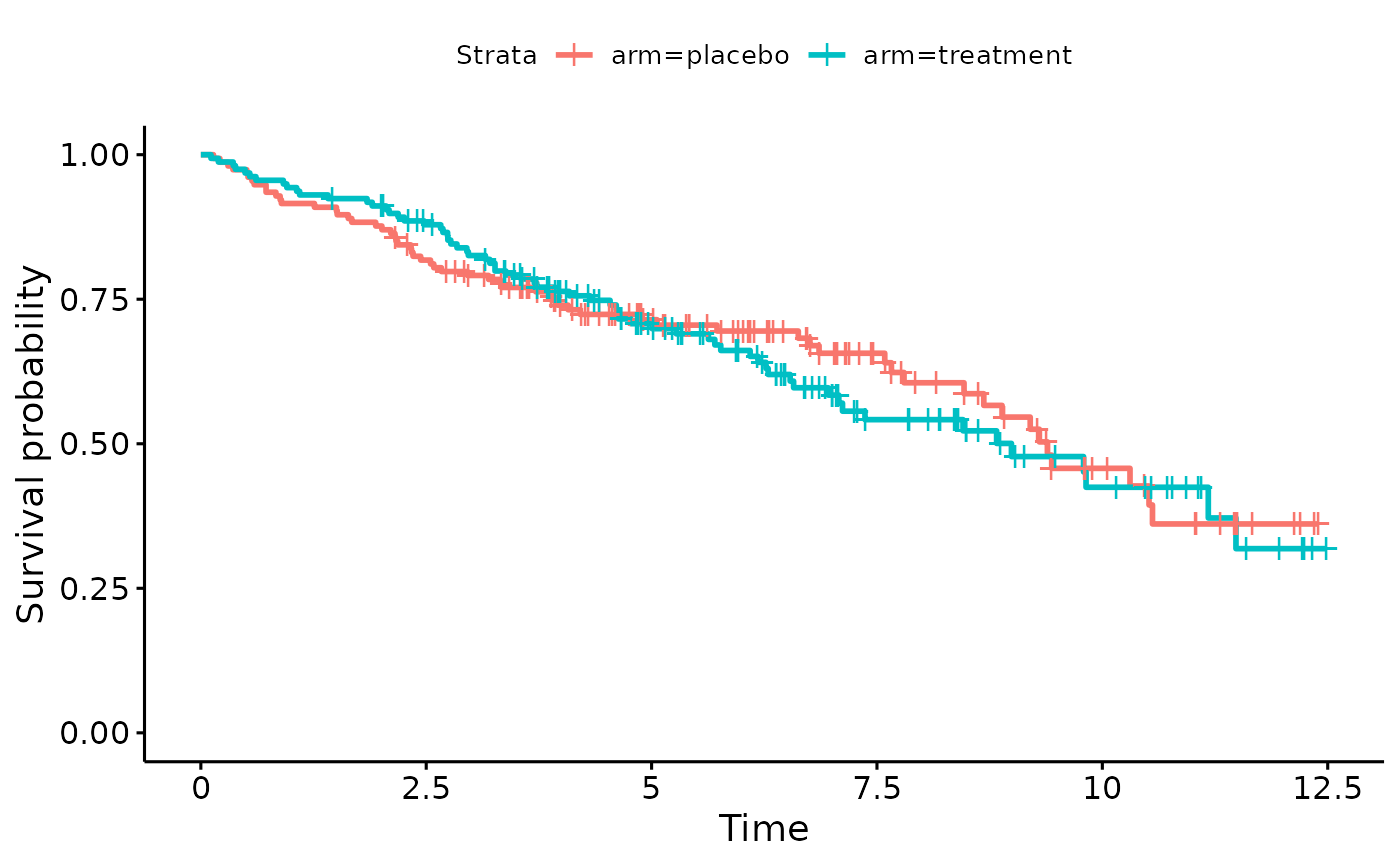
\includegraphics{../docs/articles/session_lecture_files/figure-beamer/unnamed-chunk-12-1.pdf}

\begin{verbatim}
## Warning: Vectorized input to `element_text()` is not officially supported.
## Results may be unexpected or may change in future versions of ggplot2.
\end{verbatim}

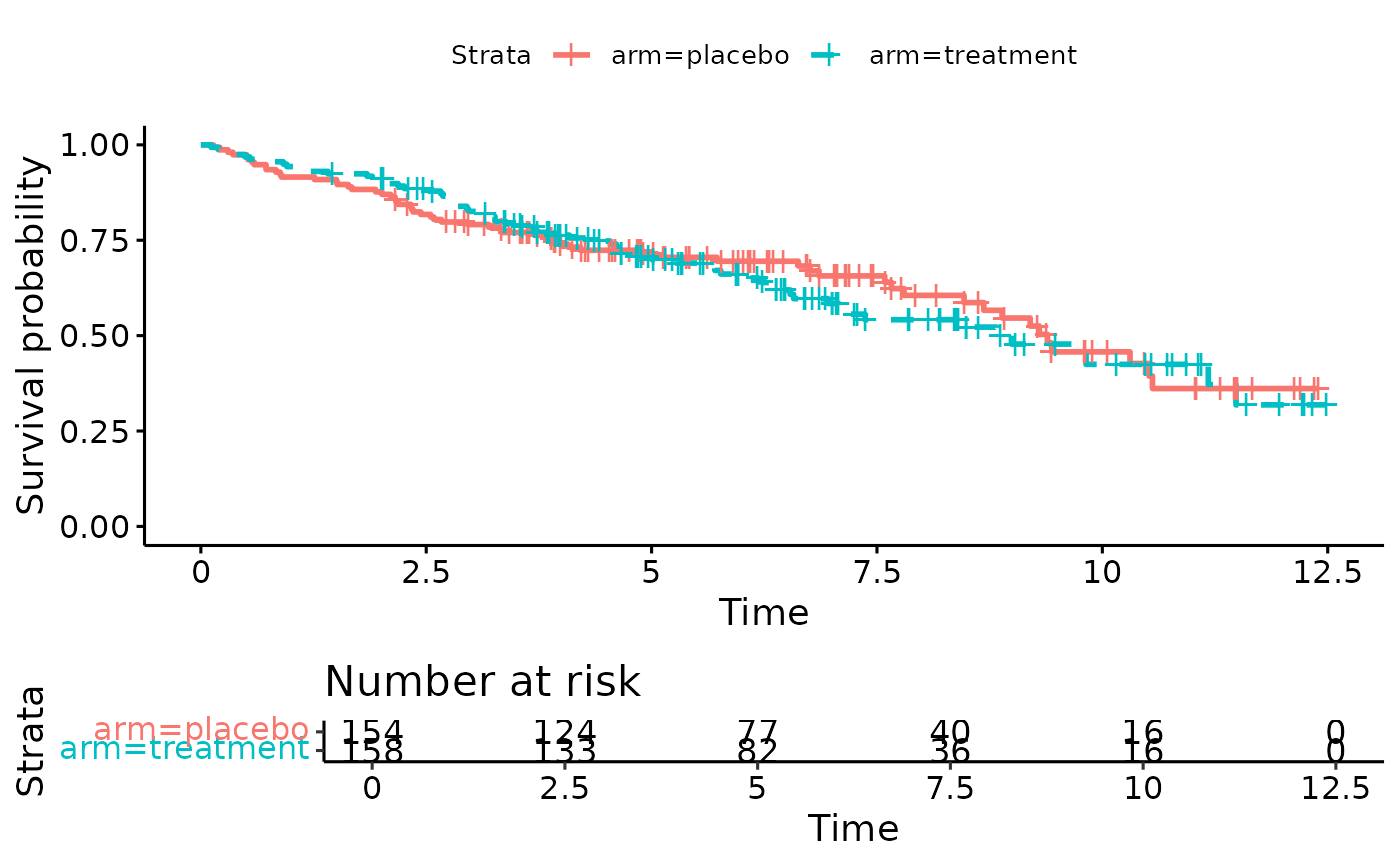
\includegraphics{../docs/articles/session_lecture_files/figure-beamer/unnamed-chunk-12-2.pdf}

\end{frame}

\hypertarget{tests-for-trend}{%
\section{Tests for trend}\label{tests-for-trend}}

\hypertarget{what-are-tests-for-trend}{%
\section{What are tests for trend?}\label{what-are-tests-for-trend}}

\begin{frame}[fragile]{What are tests for trend?}

\begin{itemize}
\tightlist
\item
  For any kind of multivariate model including an ordinal variable
\item
  Such as cancer stage (1, 2, 3, 4), age category, \ldots{}

  \begin{itemize}
  \tightlist
  \item
    Is there a linear / quadratic / cubic relationship between
    coefficients and their order?
  \item
    Test by LRT or Wald Test
  \end{itemize}
\end{itemize}

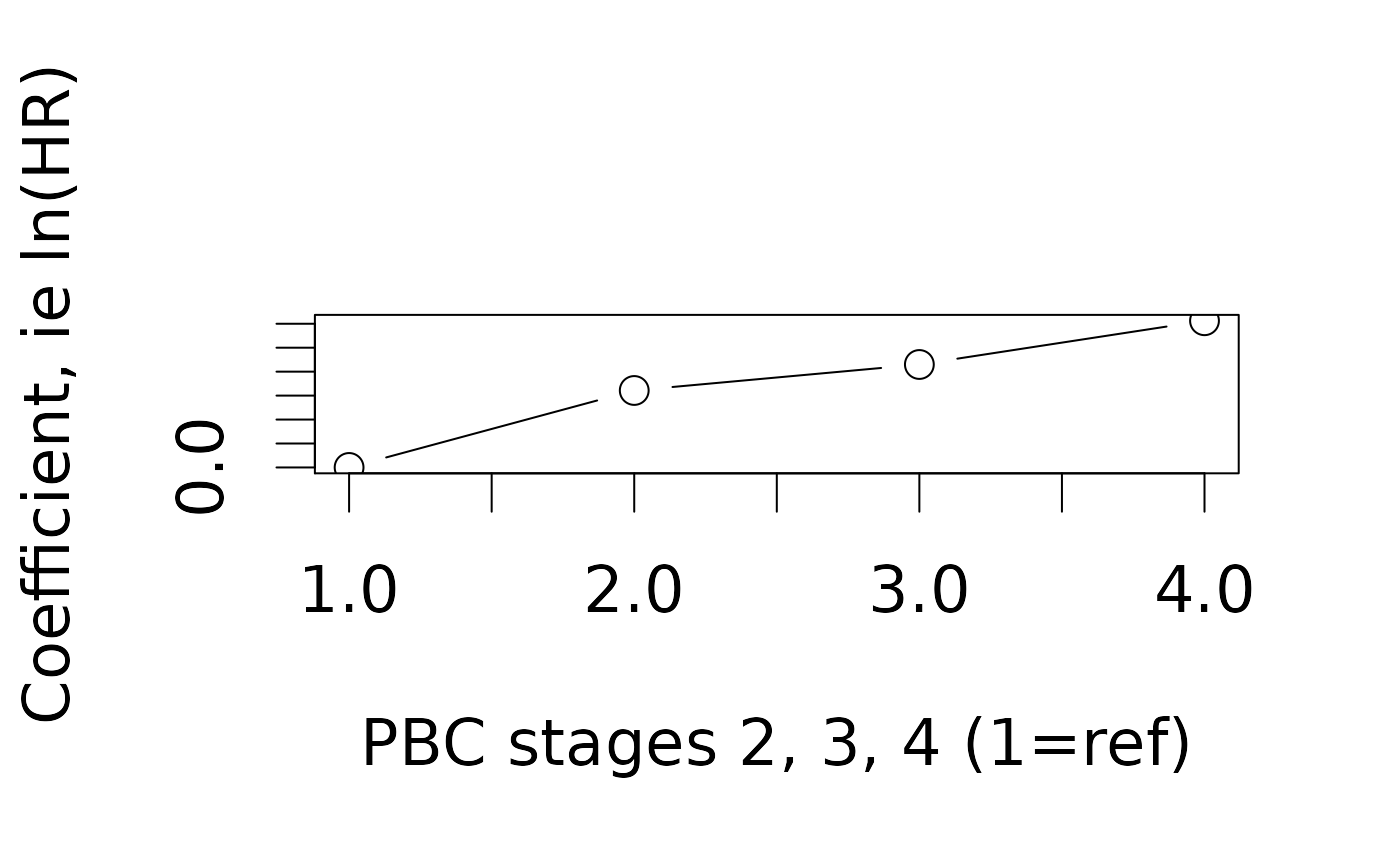
\includegraphics{../docs/articles/session_lecture_files/figure-beamer/unnamed-chunk-13-1.pdf}

\begin{verbatim}
## Call:
## coxph(formula = Surv(time, os) ~ stageordered, data = pbc.os)
## 
##   n= 312, number of events= 125 
## 
##                   coef exp(coef) se(coef)      z Pr(>|z|)   
## stageordered.L  2.1759    8.8099   0.6801  3.199  0.00138 **
## stageordered.Q -0.3469    0.7069   0.5248 -0.661  0.50867   
## stageordered.C  0.3209    1.3784   0.2990  1.073  0.28316   
## ---
## Signif. codes:  0 '***' 0.001 '**' 0.01 '*' 0.05 '.' 0.1 ' ' 1
## 
##                exp(coef) exp(-coef) lower .95 upper .95
## stageordered.L    8.8099     0.1135    2.3231    33.410
## stageordered.Q    0.7069     1.4146    0.2527     1.977
## stageordered.C    1.3784     0.7255    0.7671     2.477
## 
## Concordance= 0.702  (se = 0.022 )
## Likelihood ratio test= 52.74  on 3 df,   p=2e-11
## Wald test            = 43.92  on 3 df,   p=2e-09
## Score (logrank) test = 53.85  on 3 df,   p=1e-11
\end{verbatim}

\end{frame}

\hypertarget{predictions-for-specific-covariate-patterns}{%
\section{Predictions for specific covariate
patterns}\label{predictions-for-specific-covariate-patterns}}

\begin{frame}{How to predict survival from a Cox model?}
\protect\hypertarget{how-to-predict-survival-from-a-cox-model}{}

\begin{itemize}
\tightlist
\item
  The Cox model is a \emph{relative} risk model

  \begin{itemize}
  \tightlist
  \item
    only predicts relative risks between pairs of subjects
  \end{itemize}
\item
  Key is to calculate the overall \(S(t)\), then multiply it by the
  relative hazard for the specific covariate pattern.
\item
  In this example we plot the baseline survival for all stages together,
  then for stages 1-4 separately.
\end{itemize}

\end{frame}

\begin{frame}{Predicted survival for specific covariate patterns}
\protect\hypertarget{predicted-survival-for-specific-covariate-patterns}{}

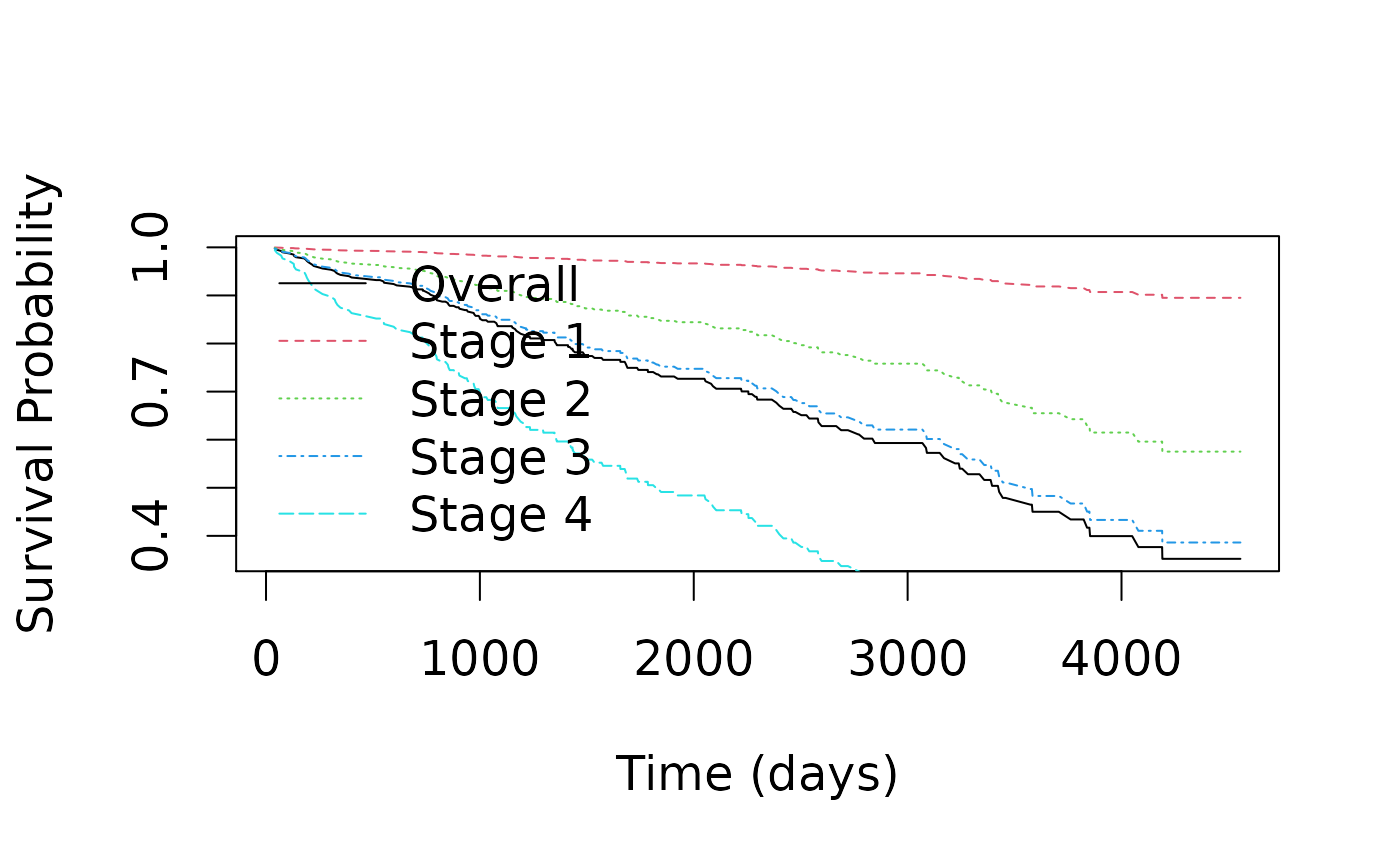
\includegraphics{../docs/articles/session_lecture_files/figure-beamer/unnamed-chunk-14-1.pdf}

\end{frame}

\begin{frame}[fragile]{Multivariate regression}
\protect\hypertarget{multivariate-regression}{}

\begin{itemize}
\tightlist
\item
  Same coding and objectives as for \texttt{lm()} and \texttt{glm()}

  \begin{itemize}
  \tightlist
  \item
    controlling for confounding
  \item
    testing for mediation
  \item
    testing for interaction
  \end{itemize}
\end{itemize}

\end{frame}

\begin{frame}[fragile]{}
\protect\hypertarget{section}{}

\tiny

\begin{Shaded}
\begin{Highlighting}[]
\NormalTok{fit <-}\StringTok{ }\KeywordTok{coxph}\NormalTok{(}\KeywordTok{Surv}\NormalTok{(time, os) }\OperatorTok{~}\StringTok{ }\NormalTok{age }\OperatorTok{+}\StringTok{ }\NormalTok{sex }\OperatorTok{+}\StringTok{ }\NormalTok{edema}
             \OperatorTok{+}\StringTok{ }\NormalTok{stage }\OperatorTok{+}\StringTok{ }\NormalTok{arm, }\DataTypeTok{data =}\NormalTok{ pbc.os)}
\KeywordTok{summary}\NormalTok{(fit)}
\end{Highlighting}
\end{Shaded}

\begin{verbatim}
## Call:
## coxph(formula = Surv(time, os) ~ age + sex + edema + stage + 
##     arm, data = pbc.os)
## 
##   n= 312, number of events= 125 
## 
##                   coef exp(coef)  se(coef)      z Pr(>|z|)    
## age           0.027618  1.028003  0.009362  2.950  0.00318 ** 
## sexf         -0.317540  0.727938  0.248839 -1.276  0.20193    
## edema0.5      0.538715  1.713804  0.275287  1.957  0.05036 .  
## edema1        2.080422  8.007845  0.276959  7.512 5.84e-14 ***
## stage2        1.535263  4.642546  1.034854  1.484  0.13793    
## stage3        1.998217  7.375893  1.016097  1.967  0.04923 *  
## stage4        2.666263 14.386101  1.016234  2.624  0.00870 ** 
## armtreatment  0.057946  1.059658  0.189200  0.306  0.75940    
## ---
## Signif. codes:  0 '***' 0.001 '**' 0.01 '*' 0.05 '.' 0.1 ' ' 1
## 
##              exp(coef) exp(-coef) lower .95 upper .95
## age             1.0280    0.97276    1.0093     1.047
## sexf            0.7279    1.37374    0.4470     1.186
## edema0.5        1.7138    0.58350    0.9992     2.940
## edema1          8.0078    0.12488    4.6534    13.780
## stage2          4.6425    0.21540    0.6108    35.288
## stage3          7.3759    0.13558    1.0067    54.040
## stage4         14.3861    0.06951    1.9630   105.430
## armtreatment    1.0597    0.94370    0.7313     1.535
## 
## Concordance= 0.77  (se = 0.022 )
## Likelihood ratio test= 107.6  on 8 df,   p=<2e-16
## Wald test            = 120.8  on 8 df,   p=<2e-16
## Score (logrank) test = 177.1  on 8 df,   p=<2e-16
\end{verbatim}

\end{frame}

\begin{frame}[fragile]{Predicted survival for adjusted coefficients}
\protect\hypertarget{predicted-survival-for-adjusted-coefficients}{}

\begin{itemize}
\tightlist
\item
  Can create Kaplan-Meier curves for crude or unadjusted coefficients

  \begin{itemize}
  \tightlist
  \item
    Section 6.3.2.3 in Vittinghoff
  \end{itemize}
\item
  Idea is to estimate hazard ratio in an unadjusted model:
\end{itemize}

\footnotesize

\begin{Shaded}
\begin{Highlighting}[]
\NormalTok{unadjfit <-}\StringTok{ }\KeywordTok{coxph}\NormalTok{(}\KeywordTok{Surv}\NormalTok{(time, os) }\OperatorTok{~}\StringTok{ }\NormalTok{stage, }\DataTypeTok{data =}\NormalTok{ pbc.os)}
\KeywordTok{coef}\NormalTok{(unadjfit)}
\end{Highlighting}
\end{Shaded}

\begin{verbatim}
##   stage2   stage3   stage4 
## 1.607014 2.149500 3.062775
\end{verbatim}

\end{frame}

\begin{frame}[fragile]{Predicted survival for adjusted coefficients
(cont'd)}
\protect\hypertarget{predicted-survival-for-adjusted-coefficients-contd}{}

\begin{itemize}
\tightlist
\item
  and in an adjusted model:
\end{itemize}

\footnotesize

\begin{Shaded}
\begin{Highlighting}[]
\NormalTok{adjfit <-}\StringTok{ }\KeywordTok{coxph}\NormalTok{(}\KeywordTok{Surv}\NormalTok{(time, os) }\OperatorTok{~}\StringTok{ }\NormalTok{age }\OperatorTok{+}\StringTok{ }\NormalTok{sex }\OperatorTok{+}\StringTok{ }\NormalTok{edema}
                \OperatorTok{+}\StringTok{ }\NormalTok{stage }\OperatorTok{+}\StringTok{ }\NormalTok{arm, }\DataTypeTok{data =}\NormalTok{ pbc.os)}
\KeywordTok{coef}\NormalTok{(adjfit)}
\end{Highlighting}
\end{Shaded}

\begin{verbatim}
##          age         sexf     edema0.5       edema1       stage2       stage3 
##    0.0276179   -0.3175396    0.5387152    2.0804217    1.5352629    1.9982170 
##       stage4 armtreatment 
##    2.6662626    0.0579460
\end{verbatim}

\end{frame}

\begin{frame}{Predicted survival for adjusted coefficients (cont'd)}
\protect\hypertarget{predicted-survival-for-adjusted-coefficients-contd-1}{}

\begin{itemize}
\tightlist
\item
  The survival function will be calculated for a ``baseline'' group, say
  stage 1, then exponentiated with the adjusted coefficient, e.g.: \[
  [S_{stage=1}(t)]^{exp(\beta_{stage=4})}
  \]
\end{itemize}

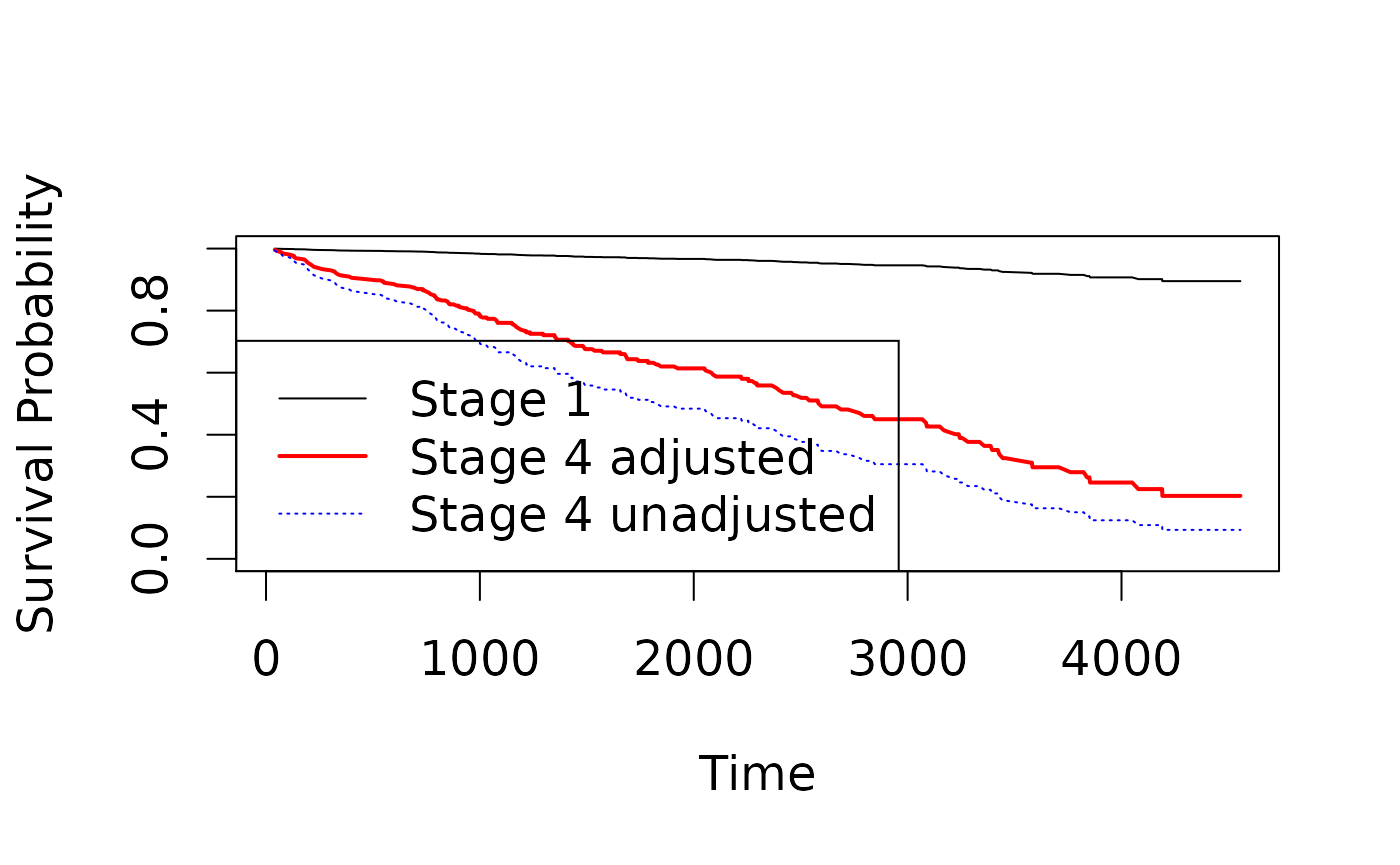
\includegraphics{../docs/articles/session_lecture_files/figure-beamer/unnamed-chunk-18-1.pdf}

\end{frame}

\hypertarget{stratification}{%
\section{Stratification}\label{stratification}}

\begin{frame}{What is stratification?}
\protect\hypertarget{what-is-stratification}{}

\begin{itemize}
\item
  relevant to all kinds of regression, not just survival analysis
\item
  when analysis is separated into groups or strata

  \begin{itemize}
  \tightlist
  \item
    must have an adequate number of events in each stratum (at least 5
    to 7)
  \item
    can be used to adjust for variables with strong impact on survival
  \item
    can help solve proportional hazards violations
  \end{itemize}
\item
  Strata have different baseline hazards
\item
  Coefficients / Hazard Ratios are calculated within stratum then
  combined.
\item
  Vittinghoff 6.3.2
\end{itemize}

\end{frame}

\begin{frame}[fragile]{How to stratify}
\protect\hypertarget{how-to-stratify}{}

\textbf{Example - in R, strata() can be added to any model formula}
\footnotesize

\begin{Shaded}
\begin{Highlighting}[]
\NormalTok{mycox <-}\StringTok{ }\KeywordTok{coxph}\NormalTok{(}\KeywordTok{Surv}\NormalTok{(time, os) }\OperatorTok{~}\StringTok{ }\NormalTok{trt }\OperatorTok{+}\StringTok{ }\KeywordTok{strata}\NormalTok{(stage), }
               \DataTypeTok{data =}\NormalTok{ pbc.os)}
\KeywordTok{summary}\NormalTok{(mycox)}
\end{Highlighting}
\end{Shaded}

\begin{verbatim}
## Call:
## coxph(formula = Surv(time, os) ~ trt + strata(stage), data = pbc.os)
## 
##   n= 312, number of events= 125 
## 
##        coef exp(coef) se(coef)      z Pr(>|z|)
## trt -0.1063    0.8992   0.1814 -0.586    0.558
## 
##     exp(coef) exp(-coef) lower .95 upper .95
## trt    0.8992      1.112    0.6302     1.283
## 
## Concordance= 0.494  (se = 0.025 )
## Likelihood ratio test= 0.34  on 1 df,   p=0.6
## Wald test            = 0.34  on 1 df,   p=0.6
## Score (logrank) test = 0.34  on 1 df,   p=0.6
\end{verbatim}

\end{frame}

\hypertarget{competing-risks-data}{%
\section{Competing Risks Data}\label{competing-risks-data}}

\begin{frame}{What are competing risks?}
\protect\hypertarget{what-are-competing-risks}{}

\begin{itemize}
\tightlist
\item
  Example from Vittinghoff 6.5: The MrOS study (Orwoll et al.~2005)
  followed men over 65 to examine predictors of bone fracture and low
  BMD (subclinical bone loss)
\item
  At end of study participants had:

  \begin{itemize}
  \tightlist
  \item
    developed fracture (outcome of interest),
  \item
    remained alive without fracture (incomplete follow-up), or
  \item
    died prior to fracture (incomplete follow-up)
  \end{itemize}
\end{itemize}

\tiny Orwoll, E. \emph{et al.} (2005). Design and baseline
characteristics of the osteoporotic fractures in men (MrOS) study--a
large observational study of the determinants of fracture in older men.
Contemporary Clinical Trials, 26(5), 569--585.

\end{frame}

\begin{frame}{Why not treat died prior to fracture and alive without
fracture as censored?}
\protect\hypertarget{why-not-treat-died-prior-to-fracture-and-alive-without-fracture-as-censored}{}

\begin{itemize}
\tightlist
\item
  Recall the independent censoring assumption (Vittinghoff 6.6.4):

  \begin{itemize}
  \tightlist
  \item
    censored people are similar to those who remain at risk in terms of
    developing the event of interest;
  \item
    censoring is independent of the event of interest.
  \item
    For patients who died this assumption is highly suspect
  \end{itemize}
\end{itemize}

\end{frame}

\begin{frame}{Reasons for right censored data}
\protect\hypertarget{reasons-for-right-censored-data}{}

\begin{itemize}
\tightlist
\item
  Cut-off date of analysis (administrative censoring):

  \begin{itemize}
  \tightlist
  \item
    Censoring usually independent
  \end{itemize}
\item
  Loss to follow-up

  \begin{itemize}
  \tightlist
  \item
    Independence may be problematic if sicker individuals discontinue
    participant in study (lack of energy, too ill, return to home
    country)
  \item
    or if healthier individuals discontinue participation (don't feel
    the need to continue, start new life in other country)
  \end{itemize}
\item
  Competing risks:

  \begin{itemize}
  \tightlist
  \item
    Often informative.
  \item
    In competing risks analysis, independence between competing risks is
    not required
  \end{itemize}
\end{itemize}

\end{frame}

\begin{frame}{Very brief summary of competing risk methods}
\protect\hypertarget{very-brief-summary-of-competing-risk-methods}{}

\begin{itemize}
\tightlist
\item
  1-to-1 mapping between hazard and cumulative incidence function is
  lost in competing risks
\item
  Standard Kaplan-Meier estimator is biased for competing risks data

  \begin{itemize}
  \tightlist
  \item
    Aalen-Johansen estimator is better choice
  \end{itemize}
\item
  \emph{Gary's test} is analogous to log-rank test
\item
  cause-specific standard Cox PH model might be useful for prognostic
  (causal) testing, but not estimating a population Hazard Ratio
\end{itemize}

\end{frame}

\begin{frame}{Resources for competing risk methods}
\protect\hypertarget{resources-for-competing-risk-methods}{}

\begin{itemize}
\tightlist
\item
  Z. Zhang, Survival analysis in the presence of competing risks, Ann
  Transl Med. 2017 Feb; 5(3): 47. PMID:
  \href{https://www.ncbi.nlm.nih.gov/pubmed/28251126}{28251126}
\item
  \href{https://CRAN.R-project.org/package=cmprsk}{cmprsk} package
\item
  \href{https://cran.r-project.org/package=riskRegression}{riskRegression}
  package
\end{itemize}

\end{frame}

\hypertarget{propensity-score-analysis}{%
\section{Propensity score analysis}\label{propensity-score-analysis}}

\begin{frame}[fragile]{What is propensity score analysis?}
\protect\hypertarget{what-is-propensity-score-analysis}{}

\begin{itemize}
\tightlist
\item
  an alternative to multivariate regression to control for hypothesized
  confounders in observational studies:
\end{itemize}

\begin{verbatim}
outcome ~ exposure + counfounder1 + confounder2
\end{verbatim}

\begin{itemize}
\tightlist
\item
  a stratification approach that is more practical than stratifying on
  multiple hypothesized confounders
\item
  an approach to summarizing many covariates into a single score
\item
  a convenient approach to controlling for many hypothesized confounders
\end{itemize}

\end{frame}

\begin{frame}[fragile]{Propensity score approach to correction for
confounders}
\protect\hypertarget{propensity-score-approach-to-correction-for-confounders}{}

\begin{itemize}
\tightlist
\item
  \emph{Step 1}: fit the propensity score model (no outcome) that
  predicts propensity for exposure based on confounders:
\end{itemize}

\begin{verbatim}
exposure ~ counfounder1 + confounder2
\end{verbatim}

\begin{itemize}
\item
  \emph{Step 2}: use propensity predictions to match or stratify
  participants with similar propensity (for example, stratifying on
  quintiles of propensity)
\item
  \emph{Step 3}: check adequacy of matching or stratification, ie by
  comparing attributes of matched participants
\item
  \emph{Step 4}: test hypothesis \emph{among matched participants}:
\end{itemize}

\begin{verbatim}
outcome ~ exposure
\end{verbatim}

\end{frame}

\begin{frame}{Propensity score references}
\protect\hypertarget{propensity-score-references}{}

\begin{itemize}
\tightlist
\item
  P.C. Austin (2011), An Introduction to Propensity Score Methods for
  Reducing the Effects of Confounding in Observational Studies.
  Multivariate Behavioral Research, 46:3, 399-424, DOI:
  \href{http://dx.doi.org/10.1080/00273171.2011.568786}{10.1080/00273171.2011.568786}
\item
  R. d'Agostino (1998), Tutorial in Biostatistics: propensity score
  methods for bias reduction in the comparison of a treatment to a
  non-randomized control group. Stat. Med. 17, 2265-2281.
  \url{http://www.stat.ubc.ca/~john/papers/DAgostinoSIM1998.pdf}
\item
  You don't need any special package to do basic propensity score
  matching (e.g.~stratifying by quintiles), but the
  \href{https://cran.r-project.org/package=MatchIt}{MatchIt} package
  provides multiple matching approaches, diagnostics, good documentation
\end{itemize}

\end{frame}

\end{document}
